\RequirePackage{ifpdf}
\documentclass[english]{lni}

% ============================================================
% Encoding and basic packages
% ============================================================

\usepackage[utf8]{inputenc}
\usepackage{graphicx}
\usepackage{amsfonts}
\usepackage{amsmath}
\usepackage{booktabs}
\usepackage{tabularx}
\usepackage{array}
\usepackage{float}
\usepackage{makecell}
\usepackage{pdflscape}
\usepackage{geometry}
\usepackage{caption}
\usepackage{enumitem}
\usepackage{xcolor}

% ============================================================
% Paths and layout helpers
% ============================================================

\graphicspath{{figures/}}

\newcolumntype{Y}{>{\raggedright\arraybackslash}X}

\setlist[itemize]{
    leftmargin=1.35em,
    itemsep=2pt,
    topsep=3pt
}

\setlist[enumerate]{
    leftmargin=1.65em,
    itemsep=2pt,
    topsep=3pt
}


% ============================================================
% Document
% ============================================================

\begin{document}

% ============================================================
% Title Page
% ============================================================

\begin{titlepage}
    \thispagestyle{empty}

    \begin{center}

        \vspace*{1.5cm}

        {\Large\bfseries Bachelor Thesis\par}

        \vspace{1.4cm}

        {\LARGE\bfseries
        A Practical Evaluation of Oversmoothing and\\[0.2cm]
        Oversquashing in Graph Neural Networks
        \par}

        \vspace{1.5cm}

        {\large Malaz Natouf\par}

        \vspace{0.35cm}

        {\large
        Learning on Graphs\\
        RWTH Aachen University\\
        Aachen, Germany\\
        \texttt{malaz.natouf@rwth-aachen.de}
        \par}

        \vfill

        {\large\textbf{Professors}\par}

        \vspace{0.15cm}

        {\large
        Prof.\ Dr.\ Christopher Morris\\
        Prof.\ Dr.\ Michael Schaub
        \par}

        \vspace{0.65cm}

        {\large\textbf{Supervisor}\par}

        \vspace{0.15cm}

        {\large Timo Stoll\par}

        \vspace{0.65cm}

        {\large\textbf{Registration Date}\par}

        \vspace{0.15cm}

        {\large 28 August 2026\par}

        \vspace{0.65cm}

        {\large\textbf{Submission Date}\par}

        \vspace{0.15cm}

        {\large\phantom{28 August 2026}\par}

        \vspace{1.3cm}

    \end{center}

\end{titlepage}

\clearpage

% ============================================================
% Abstract
% ============================================================

\begin{abstract}

% Intentionally left empty.
% The abstract will be written after the main thesis
% has been completed.

\end{abstract}


% ============================================================
% Table of Contents
% ============================================================

\clearpage
\tableofcontents
\clearpage


% ============================================================
% 1 Introduction
% ============================================================

\section{Introduction}
\label{sec:introduction}

% The introduction will be written after the main theoretical,
% methodological, and empirical chapters have been completed.


\subsection{Motivation}
\label{sec:motivation}

% To be written later.


\subsection{Research Questions}
\label{sec:research-questions}

% To be written later.


% ============================================================
% 2 Background
% ============================================================

\section{Background}
\label{sec:background}


% ============================================================
% 2.1 Message Passing and Receptive Fields
% ============================================================

\subsection{Message Passing and Receptive Fields}
\label{sec:message-passing}

A graph can be represented as $G=(V,E)$, where $V$ is the set of nodes and $E$ is the set of edges
connecting pairs of nodes. In the graph-learning setting considered in this thesis, each node $v\in V$ also has an input feature vector $\mathbf{x}_v$. A graph neural network (GNN) uses these node features and the graph structure to create learned representations of the nodes. A widely used class of GNNs follows the \emph{message-passing} principle, in which information is exchanged between adjacent nodes over a sequence of neural-network layers \cite{gilmer2017mpnn}.

Let $\mathbf{h}_v^{(l)}$ denote the representation of node $v$ after
layer $l$, where $\mathbf{h}_v^{(0)}=\mathbf{x}_v$. In a message-passing layer, node $v$ first receives information from the neighboring nodes in
$\mathcal{N}(v)$. Messages generated from neighboring nodes are then combined using an aggregation operation. The result is then used to update the representation of node $v$. Following the message-passing framework of Gilmer et al.\ \cite{gilmer2017mpnn}, this process can be written in the form

\begin{equation}
    \mathbf{m}_v^{(l+1)}
    =
    \operatorname{AGG}^{(l)}
    \left(
        \left\{
            M^{(l)}
            \left(
                \mathbf{h}_v^{(l)},
                \mathbf{h}_u^{(l)},
                \mathbf{e}_{vu}
            \right)
            \,\middle|\,
            u\in\mathcal{N}(v)
        \right\}
    \right),
    \label{eq:message-aggregation}
\end{equation}

followed by

\begin{equation}
    \mathbf{h}_v^{(l+1)}
    =
    U^{(l)}
    \left(
        \mathbf{h}_v^{(l)},
        \mathbf{m}_v^{(l+1)}
    \right).
    \label{eq:message-update}
\end{equation}

Here, $M^{(l)}$ is the message function of layer $l$, $\operatorname{AGG}^{(l)}$ combines the messages arriving from the
neighbors of $v$, and $U^{(l)}$ updates the representation of the target node. The optional vector $\mathbf{e}_{vu}$ represents features associated with the edge between nodes $v$ and $u$. Since the neighbors of a node do not have a fixed order, the aggregation should not depend on the order in which these neighbors are presented. Common examples are sum, mean or maximum aggregation. The way these functions are used may differ depending on the GNN architecture \cite{gilmer2017mpnn,hamilton2017graphsage}.

One such GNN model is GraphSAGE, which is extensively used in the experiments of this thesis and provides a concrete example of this procedure. At each layer, GraphSAGE first aggregates information from the immediate neighborhood of a node. The aggregated information is then combined with the node's own representation to obtain an updated node representation \cite{hamilton2017graphsage}. Since the neighborhood representations used at one layer were themselves constructed in the preceding layer, information can propagate recursively through the graph. Thus, the first message-passing layer can incorporate information from direct neighbors. The second layer can additionally incorporate information from two edges away, and this process continues with increasing depth. 

This recursive expansion motivates the notion of a \emph{receptive field}. For a target node, the theoretical receptive field includes all nodes whose input information may influence its representation after a given number of message-passing layers. An $L$-layer network in which messages are passed between directly connected nodes can in principle incorporate information from nodes that are at most $L$ edges away from the target node. Therefore, adding more message-passing layers allows information to travel over a larger graph distance. Xu et al.\ describe the same principle through neighborhood aggregation. After $k$ iterations, the representation can use structural information rooted at the target node up to depth $k$ \cite{xu2018jk}. Figure~\ref{fig:receptive-field} illustrates this expansion for successive message-passing layers.

\begin{figure}[H]
    \centering

    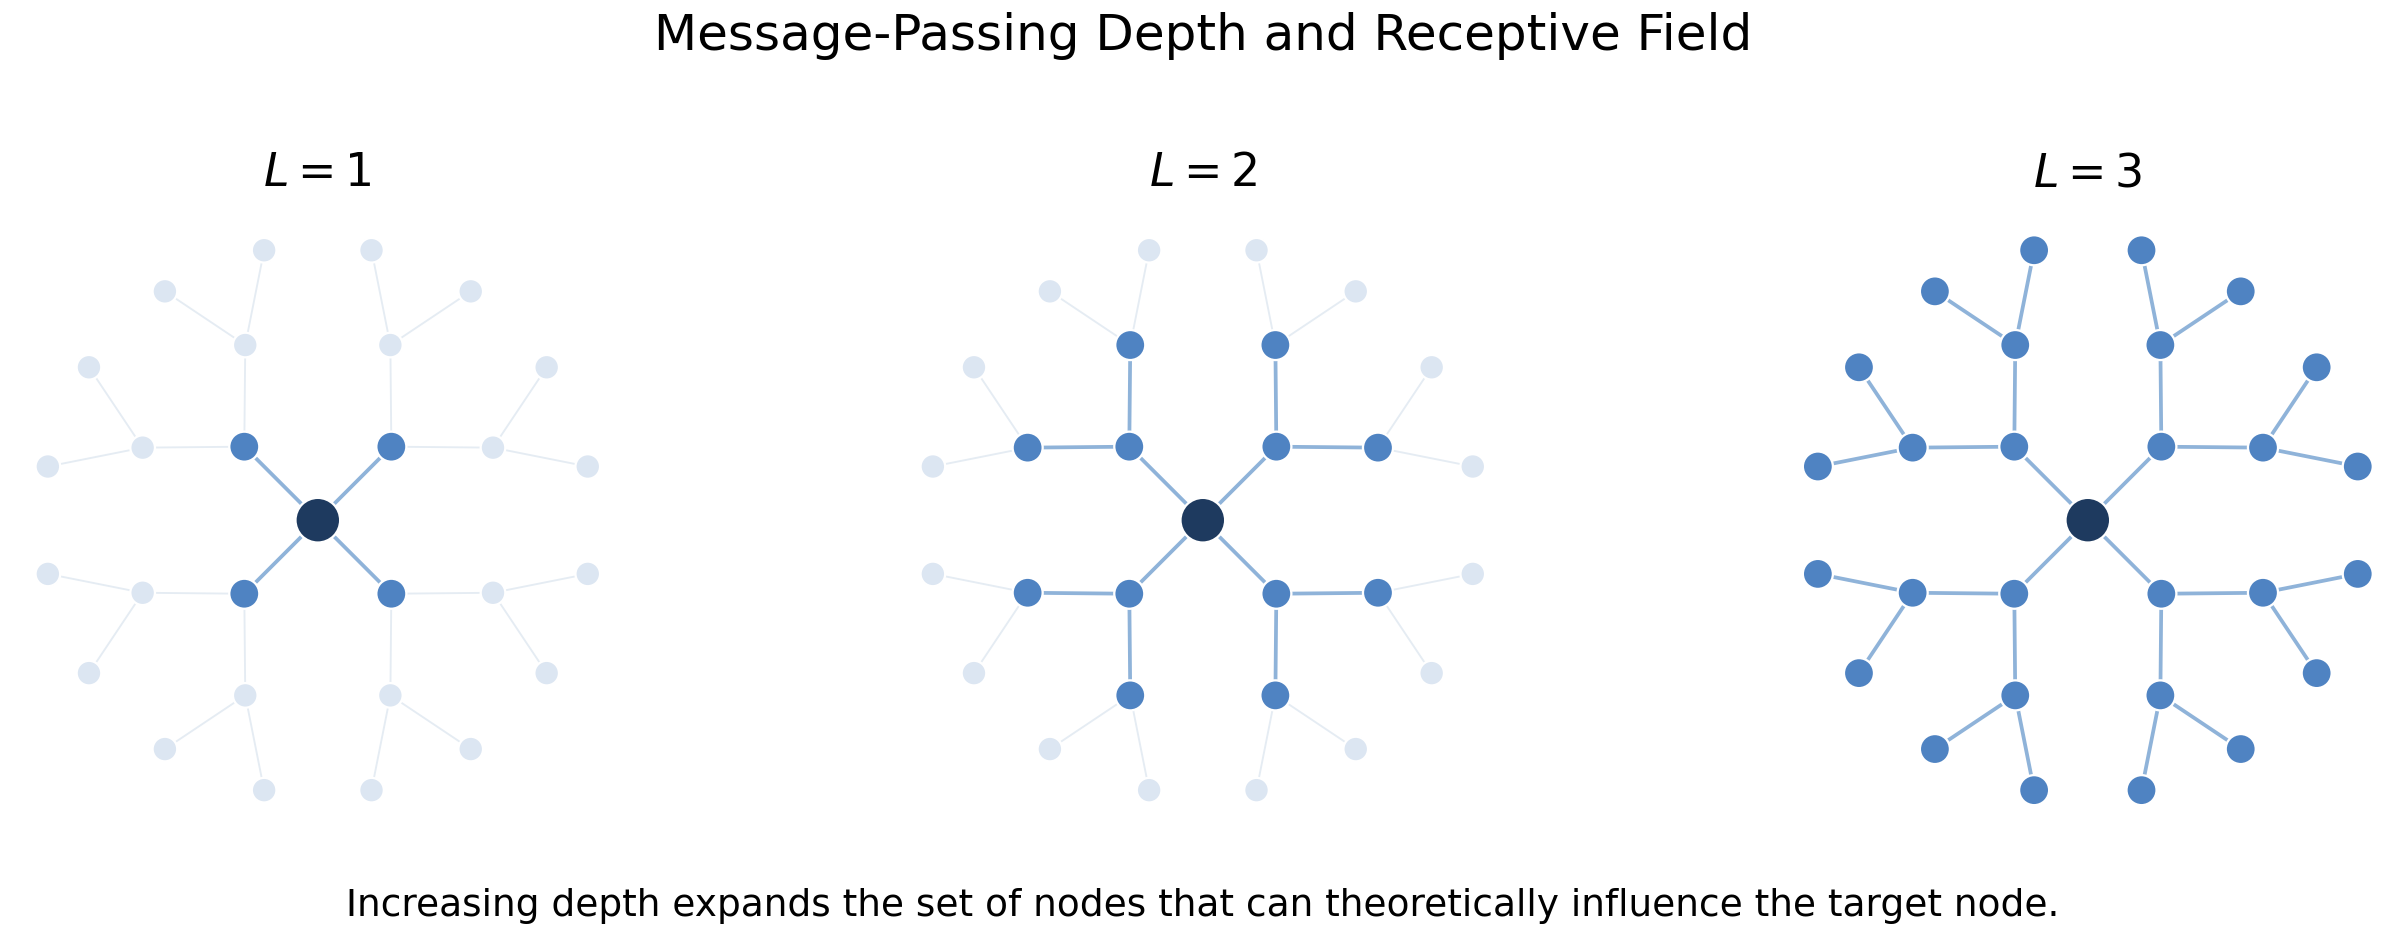
\includegraphics[
        width=0.95\textwidth,
        keepaspectratio
    ]{fig01_receptive_field.png}

    \caption{
        Receptive-field growth under repeated message passing.
        Each additional message-passing layer increases the maximum
        graph distance from which information can potentially reach
        the target node.
    }

    \label{fig:receptive-field}
\end{figure}

The theoretical receptive field should, however, be distinguished from the amount of information that actually influences a learned representation. For example, a node can be inside the $L$-hop neighborhood because a path to the target exists within $L$ message-passing steps. However, this does not mean that all nodes in this neighborhood have the same influence. The learned parameters, aggregation operation, nonlinearities, graph structure and possible neighborhood sampling determine the strength of the influence from different nodes on the final representation. Xu et al.\ formalize this distinction by studying the sensitivity of a target representation to features at other nodes and show that the effective range of influence depends strongly on the local graph structure \cite{xu2018jk}. Therefore, two target nodes processed by networks of the same depth can have the same maximum hop range while exhibiting substantially different effective information propagation.

This distinction is central to the remainder of this thesis. Increasing depth provides a larger theoretical receptive field and therefore creates the possibility of incorporating information from more distant parts of a graph. It does not, by itself, guarantee that this information is preserved or used effectively. The following sections therefore separate the number of propagation steps from the capacity of the intermediate representations and subsequently examine how repeated message passing can affect the geometry and usefulness of node representations.

% ============================================================
% 2.2 Depth versus Hidden Dimension
% ============================================================

\subsection{Depth versus Hidden Dimension}
\label{sec:depth-width}

The previous section established that stacking message-passing layers increases the maximum graph distance over which information can potentially reach a target node. Network depth therefore determines how many propagation steps are possible. Nevertheless, the information that a graph neural network can represent is not determined by its depth alone. Another key architectural factor is the dimensionality of the intermediate node representations, often referred to as the \emph{hidden dimension} or network width.

Using the notation from Section ~\ref{sec:message-passing}, let the representation of node $v$ at layer $l$ be $\mathbf{h}_v^{(l)}$. If the hidden representation contains $p$ components, then

\begin{equation}
    \mathbf{h}_v^{(l)} \in \mathbb{R}^{p}.
    \label{eq:hidden-dimension}
\end{equation}

Network depth $L$ and hidden dimension $p$ describe two different aspects of the network. Depth specifies how many successive message-passing steps are applied. In architectures based on local one-hop message passing, greater depth means information can propagate over larger distances, thereby expanding the theoretical receptive field. Hidden dimension, on the other hand, specifies the size of the vector used to store and transform a node’s intermediate representation. Therefore, increasing $p$ does not add another propagation step, which means it does not extend the receptive field \cite{loukas2020depthwidth}.

This difference is illustrated in Figure~\ref{fig:depth-width}. Increasing depth adds further message-passing layers, resulting in information passing through additional edges before the final representation is obtained. By contrast, increasing the hidden dimension enlarges the intermediate representation available at each layer. The two changes can therefore influence the model in different ways. One changes the number of communication steps through the graph, whereas the other changes the dimensionality of the state carried through those steps. Throughout this thesis, the term \emph{hidden dimension} refers to the common dimensionality assigned to the intermediate hidden representations.

The distinction between these quantities is also relevant from an expressive-power perspective. Loukas studies message-passing graph neural networks under explicit restrictions on depth and width and shows that, for several graph problems in the considered theoretical setting, restricting these parameters limits the computational power of the network \cite{loukas2020depthwidth}. The resulting bounds reveal a trade-off between depth and width for these problems, but they do not imply that the two architectural parameters are generally interchangeable. The theoretical analysis derives worst-case lower bounds under a defined computational model. Despite the identified trade-off, depth and width remain distinct architectural properties. While depth specifies the number of graph-local communication rounds, width governs the dimensionality of the intermediate representations.

This difference is especially relevant when information from distant nodes must be preserved across several message-passing steps. Increasing the hidden dimension provides more space for intermediate representations but does not shorten the paths along which information travels. Conversely, increasing depth enables the network to gather information from nodes that are further away without changing the size of the hidden representations. Di Giovanni et al.\ analyze these effects separately in the context of long-range information propagation and show that increasing width and increasing depth can have fundamentally different effects on the sensitivity of message-passing neural networks to distant node information \cite{digiovanni2023oversquashing}. Their findings also highlight that increasing network depth cannot generally compensate for a limited representation width. Therefore, when comparing shallow and deep graph neural networks, it is important to distinguish between the impact of additional message-passing steps and changes in the dimensionality of node representations.

This thesis follows that distinction throughout the empirical analysis. Network depth is varied to investigate the effects of successive message-passing steps, whereas the hidden dimension is recorded or controlled independently. Separating these two architectural factors is necessary for understanding whether performance differences in deeper networks can be attributed to graph structure, representation geometry, or other characteristics of the learning task.

\begin{figure}[H]
    \centering

    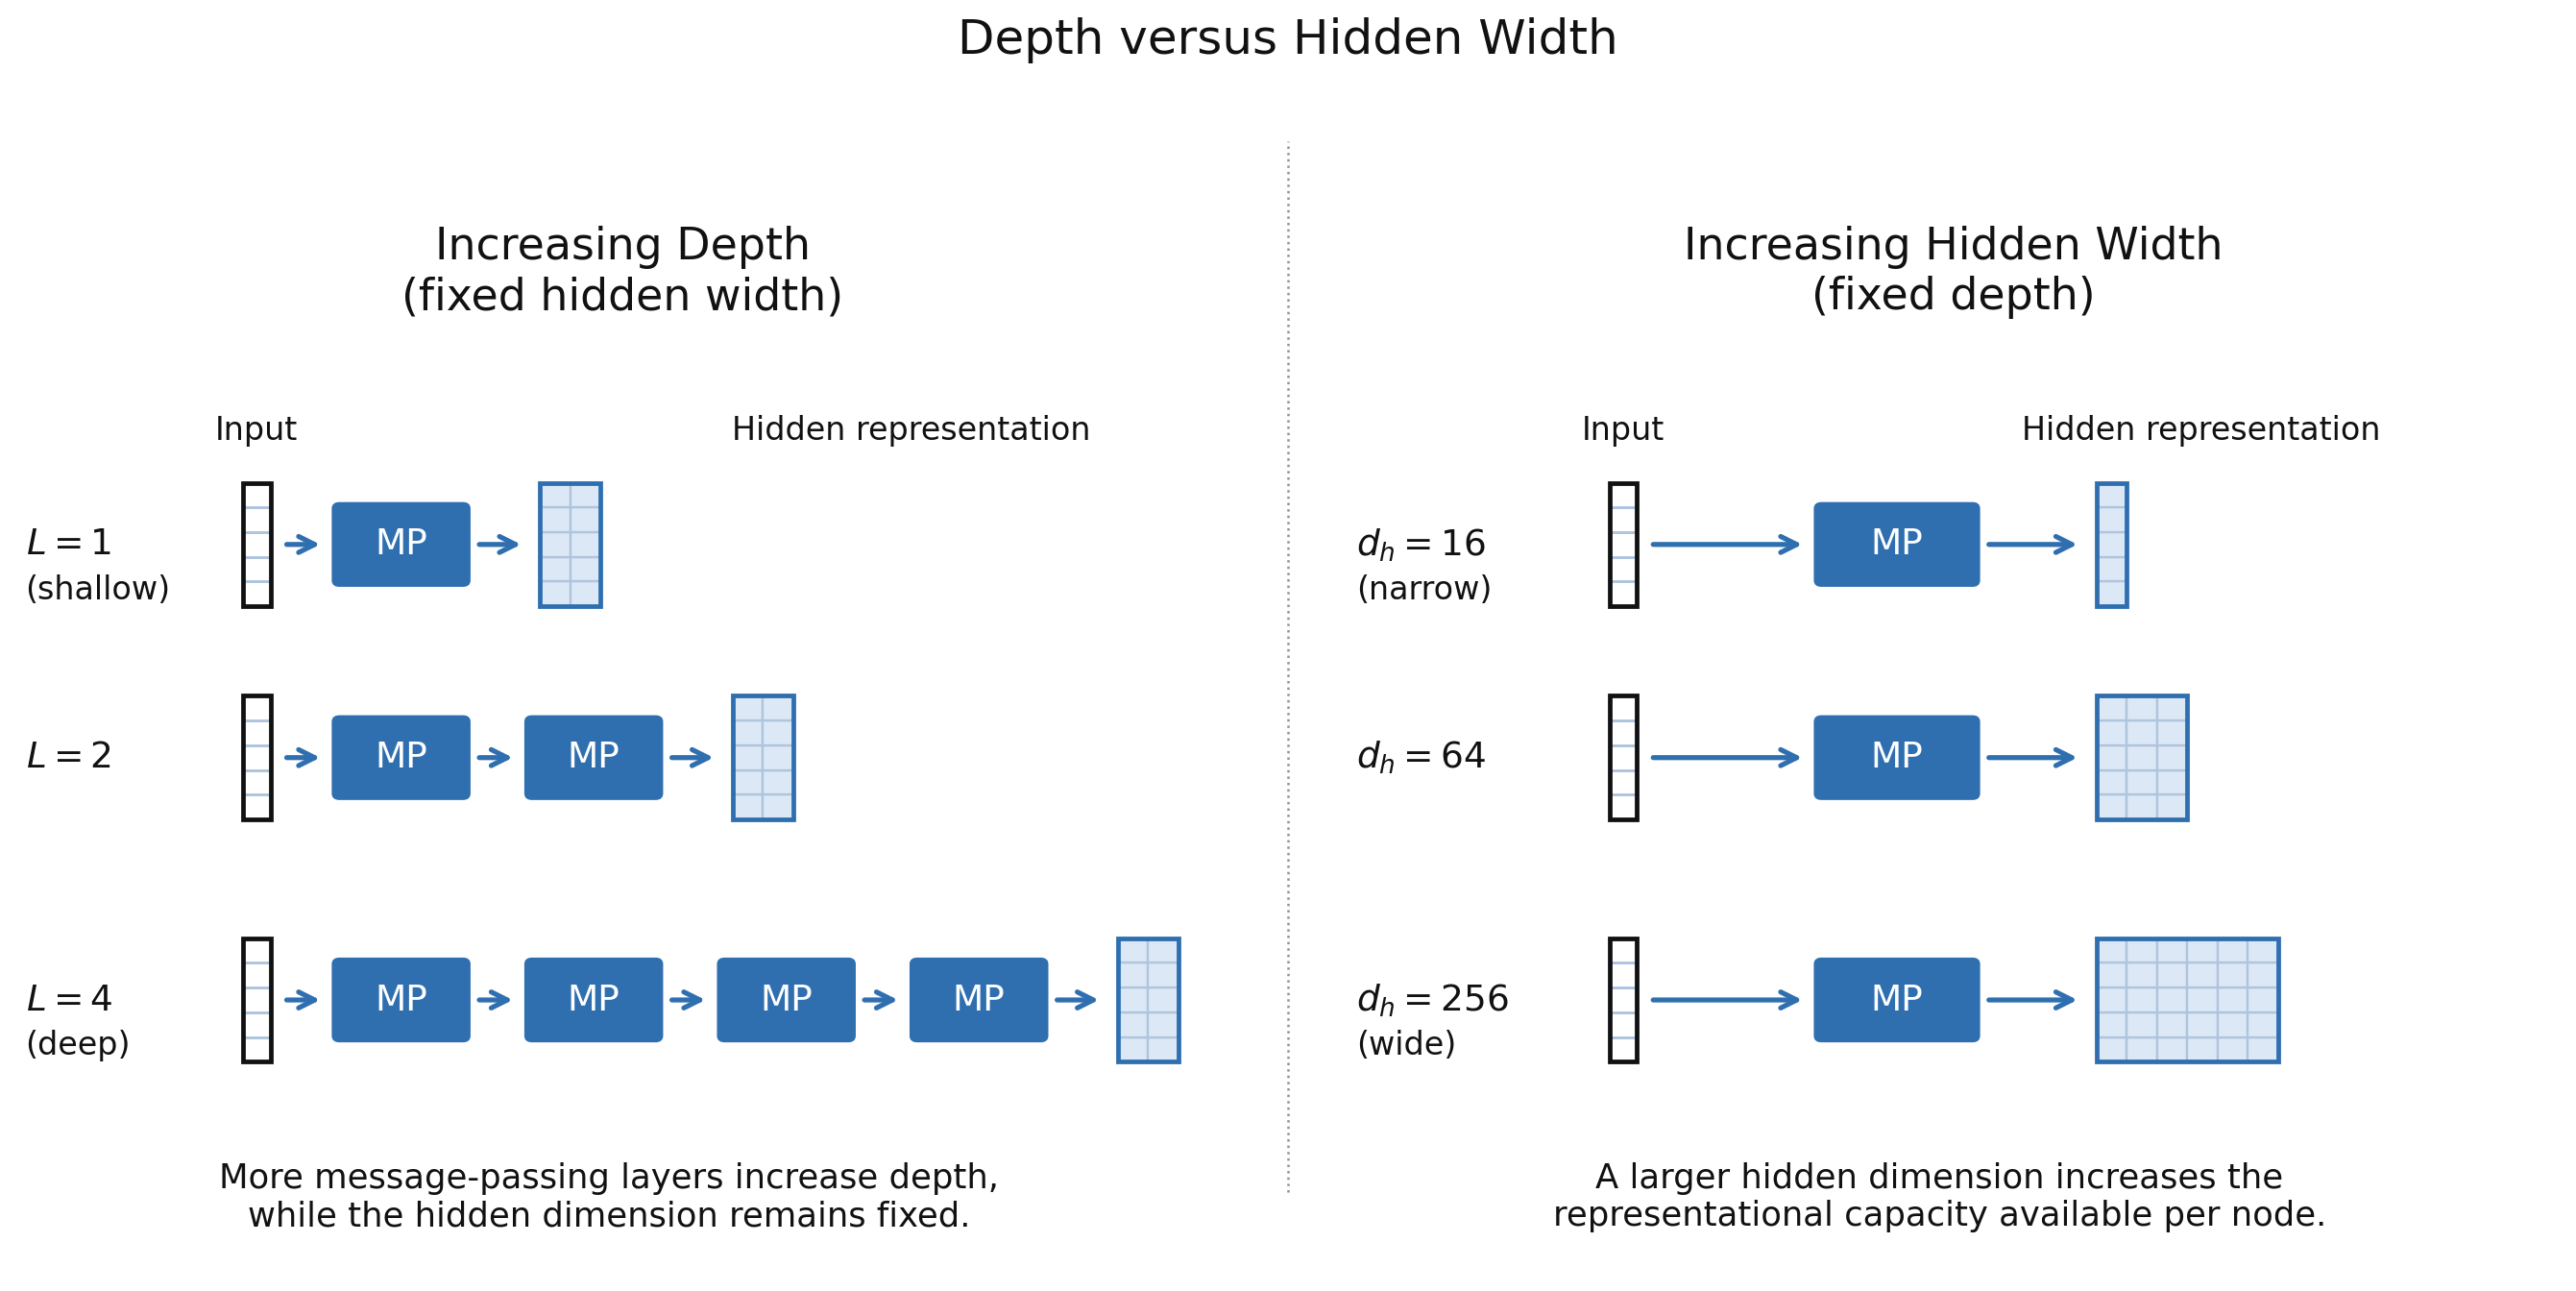
\includegraphics[
        width=0.95\textwidth,
        keepaspectratio
    ]{fig02_depth_vs_width.png}

\caption{
    Conceptual distinction between depth and hidden dimension in a
    message-passing graph neural network. Increasing depth adds
    successive propagation steps and expands the theoretical
    receptive field, whereas increasing the hidden dimension enlarges
    the intermediate node representation without adding another
    message-passing step.
}
    \label{fig:depth-width}
\end{figure}


% ============================================================
% 2.3 Homophily and Heterophily
% ============================================================

\subsection{Homophily and Heterophily}
\label{sec:homophily-heterophily}

The previous sections provided an overview of how message passing enables information to propagate between nodes in a graph and how network depth and hidden dimension influence different aspects of the GNN architecture. However, the usefulness of information aggregated from neighboring nodes also depends on the relation between the graph topology and the learning task. In node classification, this relation is often described in terms of \emph{homophily} and \emph{heterophily}.

In general, homophily describes a tendency of connected nodes to be similar, whereas heterophily describes a tendency of connected nodes to be dissimilar. The notion of similarity must be specified explicitly, since it may refer to class labels, node features, or other node attributes. In the graph-learning literature and in the experiments of this thesis, the term is primarily used with respect to class labels \cite{zhu2020heterophily,arnaiz2026demystifying}. Accordingly, a graph is more class-homophilous if connections frequently occur between nodes of the same class. In contrast, it is more class-heterophilous when edges frequently connect nodes belonging to different classes.

A simple measure of this property is the \emph{edge homophily ratio}.
For a graph $G=(V,E)$ with class label $y_v$ assigned to each node
$v$, it is defined as

\begin{equation}
    h_{\mathrm{edge}}
    =
    \frac{
        \left|
            \left\{
                (u,v)\in E
                \mid
                y_u = y_v
            \right\}
        \right|
    }{|E|}.
    \label{eq:edge-homophily}
\end{equation}

The value $h_{\mathrm{edge}}$ therefore represents the fraction of
edges whose endpoints have the same class label
\cite{zhu2020heterophily,platonov2023critical}. Values close to one
indicate that most edges are within classes, while values close to
zero indicate that most edges connect nodes from different classes.
Unless stated otherwise, the symbol $h$ in this thesis refers to this
raw class-label edge homophily measure.

The relation to message passing becomes intuitive when considering the aggregation mechanism introduced in
Section~\ref{sec:message-passing}. In a strongly homophilous graph, nodes typically aggregate information from neighbors that share the same class label. If their features also contain class-relevant information, the aggregation process can strengthen the signals relevant to the classification task.
In a heterophilous graph, nodes often have neighbors belonging to different classes. Depending on the node features and task conditions, directly mixing these representations can make class-relevant information harder to separate. This observation helps explain why many graph neural network architectures and benchmarks have historically been associated with a homophily assumption and why specialized methods have been developed to address heterophilous graphs \cite{zhu2020heterophily}.

Figure~\ref{fig:homophily-heterophily} illustrates this distinction at the level of class labels. In the homophilous example, most edges
connect nodes with the same class, whereas the heterophilous example contains a larger proportion of cross-class edges. The figure should
be interpreted as an illustration of label--topology alignment rather than as a statement about task difficulty. In particular, the fact
that neighboring nodes often belong to different classes does not imply that their relation is uninformative.

\begin{figure}[H]
    \centering

    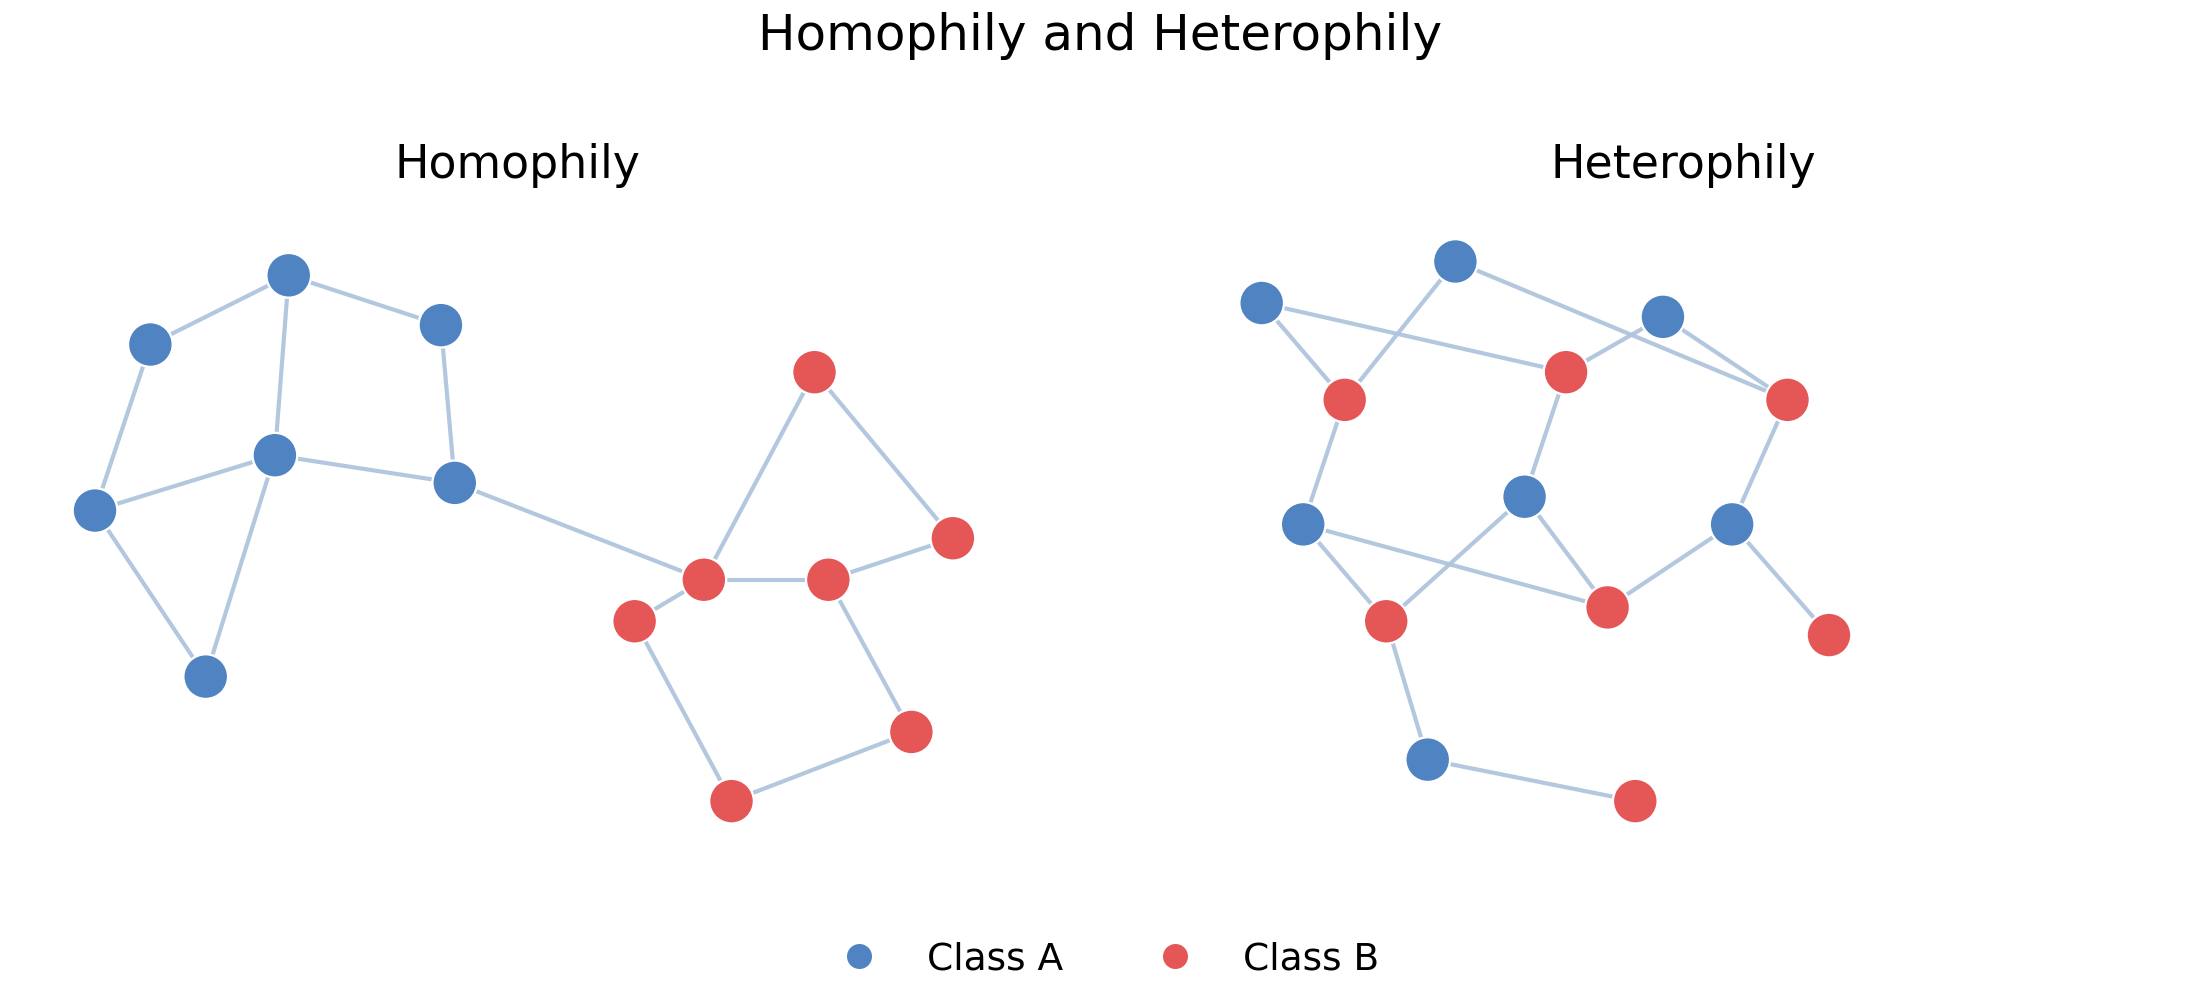
\includegraphics[
        width=0.95\textwidth,
        keepaspectratio
    ]{fig03_homophily_heterophily.png}

    \caption{
        Schematic comparison of class-homophilous and
        class-heterophilous graph structure. In the homophilous
        example, edges predominantly connect nodes of the same class,
        whereas the heterophilous example contains a larger
        proportion of edges between different classes. The schematic
        illustrates label--topology alignment and does not imply that
        one of the two settings is inherently easier to learn.
    }

    \label{fig:homophily-heterophily}
\end{figure}

This distinction is important because homophily describes the relationship between graph structure and the learning task rather than directly measuring how well a graph neural network will perform. Empirical studies have shown that standard GNNs can achieve strong predictive performance on some heterophilous graphs, while high homophily alone does not guarantee that a particular node-classification task is easy \cite{platonov2023critical,arnaiz2026demystifying}. The usefulness of neighborhood aggregation depends on additional factors, including the node features, the relationship between features and labels, the specific connectivity pattern, the learning objective, and the architecture used to process the graph.

A further limitation is that raw edge homophily should not be treated as an absolute measure that is directly comparable across arbitrary datasets. In particular, the fraction of same-class edges is affected by the number and relative sizes of the classes. Platonov et al. therefore distinguish raw edge homophily from adjusted measures that account for the amount of same-class connectivity expected from the class and degree distribution \cite{platonov2023critical}. This thesis nevertheless uses raw edge homophily when a direct and interpretable fraction of same-label edges is required, especially in the controlled experiments where target values of $h$ are imposed explicitly. Adjusted homophily is used as a supporting diagnostic where appropriate rather than as a replacement for the controlled variable. 

In this thesis, homophily and heterophily are therefore used to describe how labels align with graph structure, not as a sufficient explanation for model behavior. Arnaiz-Rodriguez and Errica similarly caution against the universal claim that homophily is inherently beneficial and heterophily inherently detrimental, emphasizing instead the interaction between the task, features, labels, and topology \cite{arnaiz2026demystifying}. This distinction is particularly relevant for the experiments presented later in this thesis, where homophily is varied under controlled conditions to examine whether differences in label–topology alignment are associated with changes in depth-related performance degradation and learned node representations.

% ============================================================
% 2.4 Oversmoothing
% ============================================================

\subsection{Oversmoothing}
\label{sec:oversmoothing-background}

Repeated message passing does not only enlarge the receptive field of
a node. It also repeatedly mixes node representations with information
from their neighborhoods. As discussed in the previous section, this
mixing can be useful when neighboring nodes contain task-relevant
information. However, if the aggregation is applied repeatedly, node
representations can become progressively less distinguishable. This
phenomenon is commonly referred to as \emph{oversmoothing}
\cite{li2018oversmoothing,rusch2023oversmoothing}.

An early explanation of this effect was given by Li et al.\
\cite{li2018oversmoothing} for graph convolutional networks. They
show that the propagation operation of a graph convolutional network
can be interpreted as a form of Laplacian smoothing. In this view,
each propagation step combines the representation of a node with
representations from its neighborhood. A moderate amount of such
smoothing can be beneficial because related nodes may obtain more
similar representations. Repeated smoothing, however, can eventually
remove distinctions that are necessary for separating nodes in the
embedding space. Oversmoothing therefore refers to excessive
representation smoothing rather than to neighborhood aggregation
itself.

Let
\[
    H^{(l)}
    =
    \begin{bmatrix}
        (\mathbf{h}_1^{(l)})^\top \\
        \vdots \\
        (\mathbf{h}_{|V|}^{(l)})^\top
    \end{bmatrix}
\]
denote the matrix containing all node representations at layer $l$.
A frequently used way of quantifying how strongly neighboring node
representations differ is the graph Dirichlet energy. In a simplified
unnormalized form, it can be written as

\begin{equation}
    E\!\left(H^{(l)}\right)
    =
    \frac{1}{2}
    \sum_{(u,v)\in E}
    \left\|
        \mathbf{h}_u^{(l)}
        -
        \mathbf{h}_v^{(l)}
    \right\|_2^2 .
    \label{eq:dirichlet-energy}
\end{equation}

A large value indicates that neighboring nodes can still have
substantially different representations, whereas a value approaching
zero indicates that representations connected by graph edges are
becoming increasingly similar. Dirichlet-energy-based measures are
therefore widely used as diagnostics of oversmoothing
\cite{rusch2023oversmoothing}. The exact normalized Dirichlet energy
used in the experiments of this thesis is defined later in
Section~\ref{sec:oversmoothing-diagnostics}, since normalization is
important when representation magnitudes differ across models or
training conditions.

The literature contains several related definitions and measures of
oversmoothing. Rusch et al.\ \cite{rusch2023oversmoothing} provide a
unified formulation in which oversmoothing is characterized by the
layer-wise exponential convergence of a suitable node-similarity
measure toward its collapsed value. This definition emphasizes that
oversmoothing is not merely the observation that two neighboring
representations happen to become slightly more similar. Rather, it
describes a systematic loss of representation diversity as network
depth increases. Other analyses characterize the limiting
representations differently depending on the propagation operator.
For example, Oono and Suzuki show that, under specific conditions on
the graph spectrum and weight matrices, deep graph convolutional
networks approach a restricted subspace at an exponential rate
\cite{oono2020oversmoothing}. Within that subspace, the remaining
information can be insufficient for distinguishing nodes that belong
to the same connected component and have the same degree.

These asymptotic results are useful for understanding the mechanism,
but they should not be interpreted as stating that every sufficiently
deep graph neural network must oversmooth in the same way. The
behavior depends on the propagation operator, graph topology,
parameterization, normalization, and training dynamics. Recent work
has further demonstrated that different oversmoothing diagnostics can
lead to different conclusions for the same representations. In
particular, Arnaiz-Rodriguez and Errica show that raw Dirichlet energy
can change substantially under simple rescaling even when the
underlying separability of the embeddings is not fundamentally
altered \cite{arnaiz2026demystifying}. This motivates the use of
multiple, scale-aware representation diagnostics rather than relying
on a single scalar quantity.

Figure~\ref{fig:oversmoothing-concept} illustrates the qualitative
idea considered in this thesis. Node representations that are
initially separated can move closer together as neighborhood
information is repeatedly aggregated. The figure is intentionally
conceptual: it illustrates loss of representation diversity but does
not imply that every graph, architecture, or training configuration
must follow the same trajectory.

A further distinction is essential for the empirical analysis in this
thesis. Oversmoothing describes a change in the geometry or
information content of node representations; it is not itself
equivalent to a decrease in predictive accuracy. Complete collapse to
a non-informative representation would clearly prevent a classifier
from distinguishing nodes that require different predictions.
Before such a limit is reached, however, smoothing can also remove
irrelevant variation while preserving or even improving
class-relevant separation. Conversely, predictive performance can
decrease for reasons other than oversmoothing, including optimization
difficulties, an uninformative receptive field, or a mismatch between
the graph structure and the learning task
\cite{kormann2026position,arnaiz2026demystifying}.

This distinction has received increasing attention in recent work.
Kormann et al.\ report that methods designed to mitigate
oversmoothing can preserve representation diversity without
consistently producing corresponding improvements in predictive
performance \cite{kormann2026position}. Arnaiz-Rodriguez and Errica
similarly argue that performance degradation should not be attributed
to oversmoothing by default and emphasize the separability of
task-relevant node representations as the more direct predictive
quantity \cite{arnaiz2026demystifying}. For this reason, the
experiments in this thesis evaluate predictive performance and
representation diagnostics separately. Evidence of representation
collapse is treated as support for an oversmoothing explanation only
when it is considered together with the corresponding task behavior.

The possibility that repeated message passing removes useful
representation diversity motivates methods that explicitly constrain
or restore the geometry of intermediate node representations. One
such method is PairNorm, which was proposed specifically as a
normalization-based approach for counteracting oversmoothing and is
introduced in the following section.


\begin{figure}[H]
    \centering

    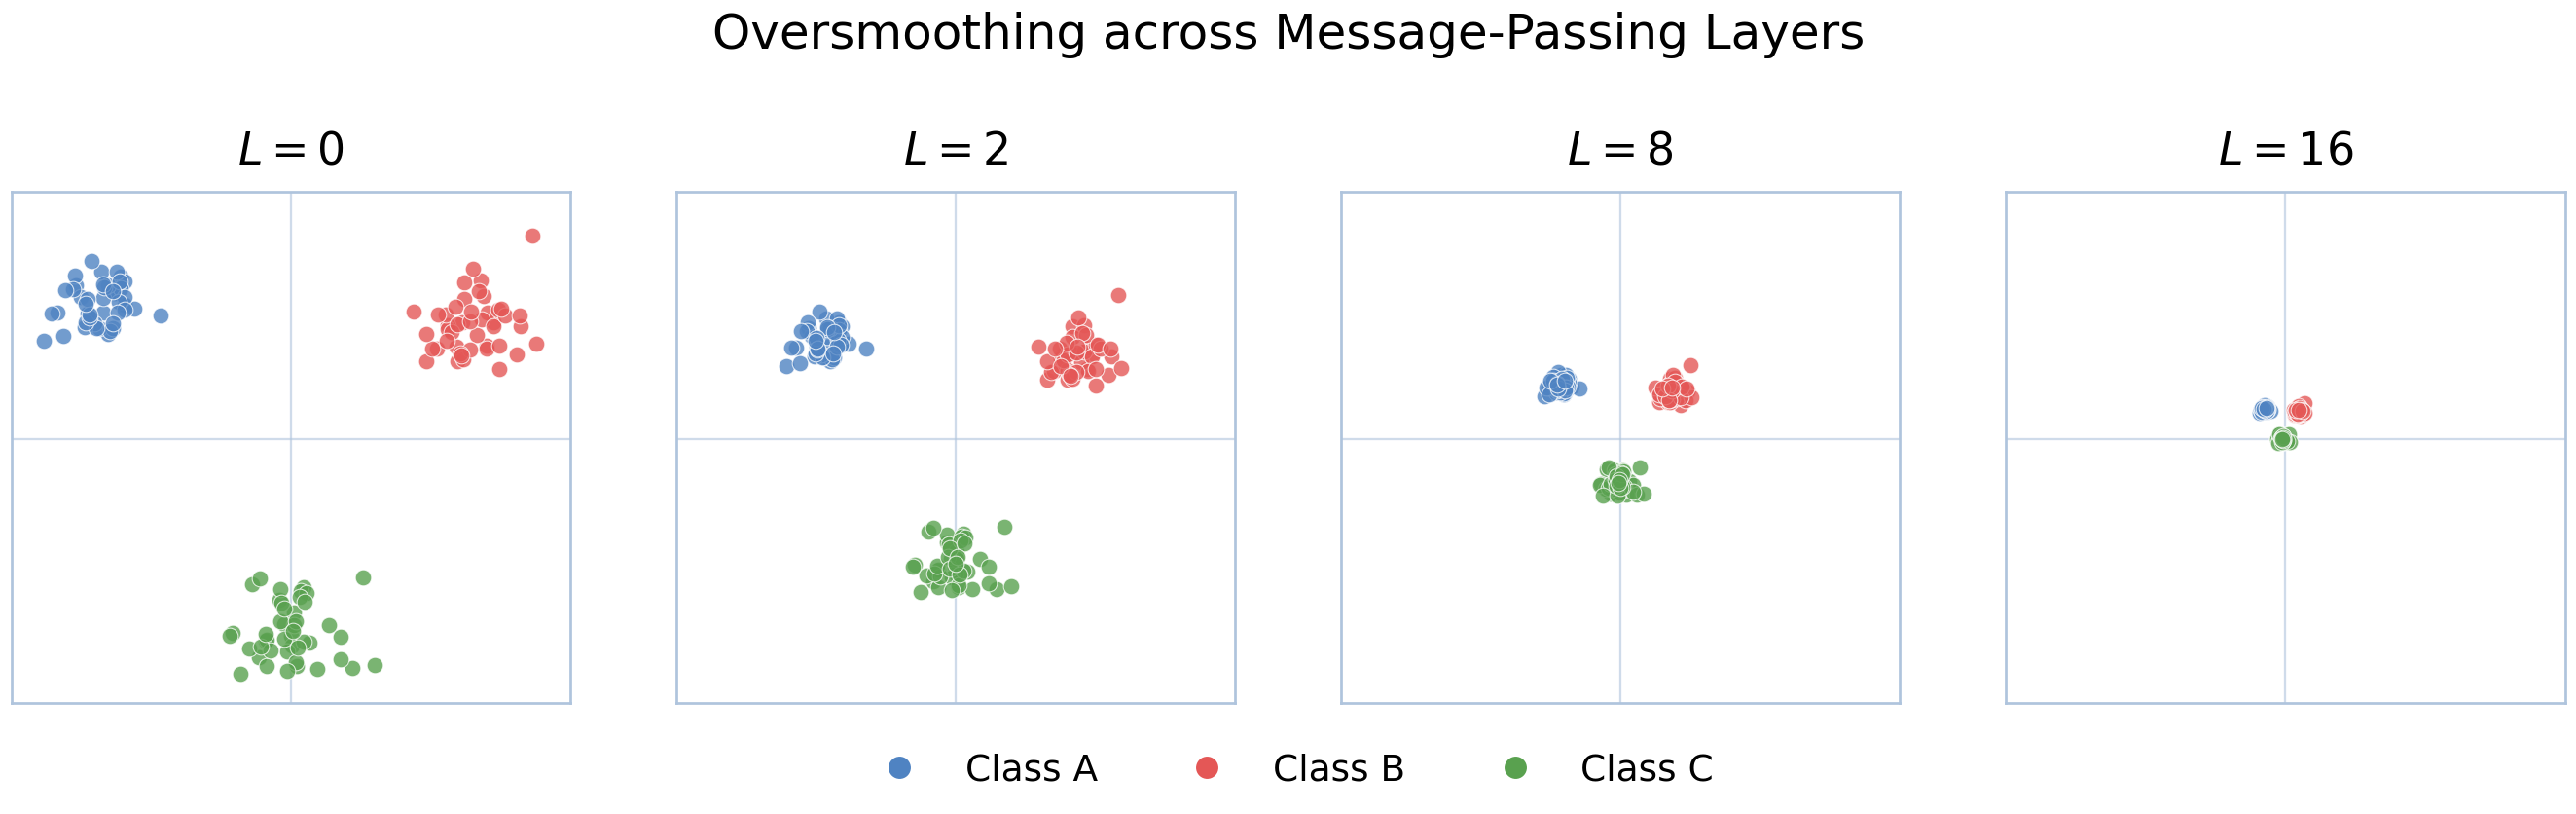
\includegraphics[
        width=0.95\textwidth,
        keepaspectratio
    ]{fig04_oversmoothing.png}

    \caption{
    Conceptual illustration of oversmoothing under repeated message
    passing. Initially distinct node representations can become
    progressively more similar as neighborhood information is
    repeatedly aggregated. The schematic illustrates representation
    collapse and does not imply that all graph neural networks
    oversmooth at the same depth or rate.
}
    \label{fig:oversmoothing-concept}
\end{figure}


% ============================================================
% 2.5 PairNorm
% ============================================================

\subsection{PairNorm}
\label{sec:pairnorm-background}

The previous section described oversmoothing as a progressive loss of
distinction between node representations under repeated message
passing. This observation motivates normalization methods that do not
prevent neighborhood aggregation itself, but constrain how strongly
the geometry of the intermediate representations can contract.
PairNorm is one such method. It was introduced by Zhao and Akoglu as
a normalization layer specifically designed to counteract
oversmoothing in graph neural networks
\cite{zhao2020pairnorm}.

The main idea of PairNorm is to control the global spread of the node
representations after a message-passing layer. Let
$\widetilde{H}\in\mathbb{R}^{n\times p}$ denote the matrix of
intermediate representations produced by such a layer, where $n$ is
the number of nodes and $p$ the hidden dimension. Its $i$-th row,
$\widetilde{\mathbf{h}}_i$, represents node $i$. Zhao and Akoglu
motivate PairNorm through the observation that repeated graph
convolution tends to decrease differences between node
representations. They therefore propose constraining the total
pairwise squared distance

\begin{equation}
    \operatorname{TPSD}(H)
    =
    \sum_{i=1}^{n}
    \sum_{j=1}^{n}
    \left\|
        \mathbf{h}_i-\mathbf{h}_j
    \right\|_2^2 ,
    \label{eq:pairnorm-tpsd}
\end{equation}

where TPSD denotes the total pairwise squared distance
\cite{zhao2020pairnorm}. Maintaining a non-vanishing global pairwise
distance prevents all node representations from simultaneously
collapsing toward the same point.

PairNorm implements this idea using two consecutive operations:
\emph{centering} and \emph{scaling}. First, the mean representation
across all nodes is removed. For each node $i$, the centered
representation is

\begin{equation}
    \widetilde{\mathbf{h}}^{\,c}_i
    =
    \widetilde{\mathbf{h}}_i
    -
    \frac{1}{n}
    \sum_{j=1}^{n}
    \widetilde{\mathbf{h}}_j .
    \label{eq:pairnorm-center}
\end{equation}

This translation moves the mean of the node representations to the
origin. Since the same vector is subtracted from every node,
centering does not change the pairwise differences between node
representations. Its purpose is instead to provide a common reference
point from which the overall scale of the representation matrix can
be controlled efficiently \cite{zhao2020pairnorm}.

The centered representations are then rescaled according to their
average squared norm. The standard PairNorm transformation can be
written as

\begin{equation}
    \mathbf{h}^{\mathrm{PN}}_i
    =
    s\,
    \frac{
        \widetilde{\mathbf{h}}^{\,c}_i
    }{
        \sqrt{
            \frac{1}{n}
            \sum_{j=1}^{n}
            \left\|
                \widetilde{\mathbf{h}}^{\,c}_j
            \right\|_2^2
        }
    },
    \label{eq:pairnorm-scale}
\end{equation}

where $s>0$ is a scale hyperparameter
\cite{zhao2020pairnorm}. After this transformation, the
representations remain centered and their total pairwise squared
distance is fixed to a value determined by $n$ and $s$. In
particular, the original PairNorm derivation gives

\begin{equation}
    \operatorname{TPSD}
    \left(
        H^{\mathrm{PN}}
    \right)
    =
    2n^2s^2 .
    \label{eq:pairnorm-tpsd-constant}
\end{equation}

PairNorm therefore does not prescribe which individual nodes should
be close to or distant from one another. Instead, it constrains the
global geometry of the complete set of node representations. Local
message passing can still make some representations more similar, but
a simultaneous collapse of all node representations is prevented by
maintaining their overall spread. This distinction is important:
PairNorm does not modify the graph topology, the receptive field, or
the number of message-passing steps. It acts only on the intermediate
representations produced by the network.

Figure~\ref{fig:pairnorm-concept} illustrates this geometric effect.
Repeated aggregation can move initially distinct node
representations toward a more concentrated region of the embedding
space. PairNorm first recenters these representations and then
rescales their global spread. The schematic should not be interpreted
as preserving every individual distance or restoring the original
positions of the nodes. Rather, it visualizes the global constraint
that prevents the complete representation set from contracting
without bound.

The original formulation is computationally simple and introduces no
additional learnable parameters. Zhao and Akoglu propose inserting
the normalization between intermediate graph neural network layers,
which allows PairNorm to be combined with different message-passing
architectures \cite{zhao2020pairnorm}. In this thesis, PairNorm is
primarily combined with GraphSAGE so that the effect of repeated
message passing can be compared with and without this normalization
under otherwise matched architectural conditions. The exact model
placement and experimental settings are specified later in the
methodology.

Preserving representation diversity, however, should not be equated
with guaranteeing higher predictive accuracy. Zhao and Akoglu
already observe that making deeper networks more robust to
oversmoothing does not necessarily improve absolute test performance
when additional depth is not useful for the underlying task
\cite{zhao2020pairnorm}. Rusch et al.\ further demonstrate that a
method can maintain a non-collapsed representation diagnostic while
predictive performance still deteriorates with increasing depth
\cite{rusch2023oversmoothing}. PairNorm is therefore treated in this
thesis as an intervention on representation geometry rather than as
an assumed solution to depth-related performance degradation.

This distinction also motivates a later component ablation. Since the
standard PairNorm transformation consists of both centering and
scaling, the experiments additionally evaluate a center-only and a
scale-only operation to determine which component is associated with
the observed changes in representation geometry and predictive
performance. These two configurations are diagnostic variants
introduced for this thesis; they should not be interpreted as
separate methods proposed in the original PairNorm work.

Finally, PairNorm is also reused later in the long-range information
propagation experiments. Its role there remains that of a
non-structural normalization intervention: unlike graph rewiring,
PairNorm does not introduce new edges or shorten graph distances.
This makes it possible to examine whether changes in long-range
behavior necessarily require a structural modification of the graph,
without redefining PairNorm as an oversquashing-specific method.


\begin{figure}[H]
    \centering

    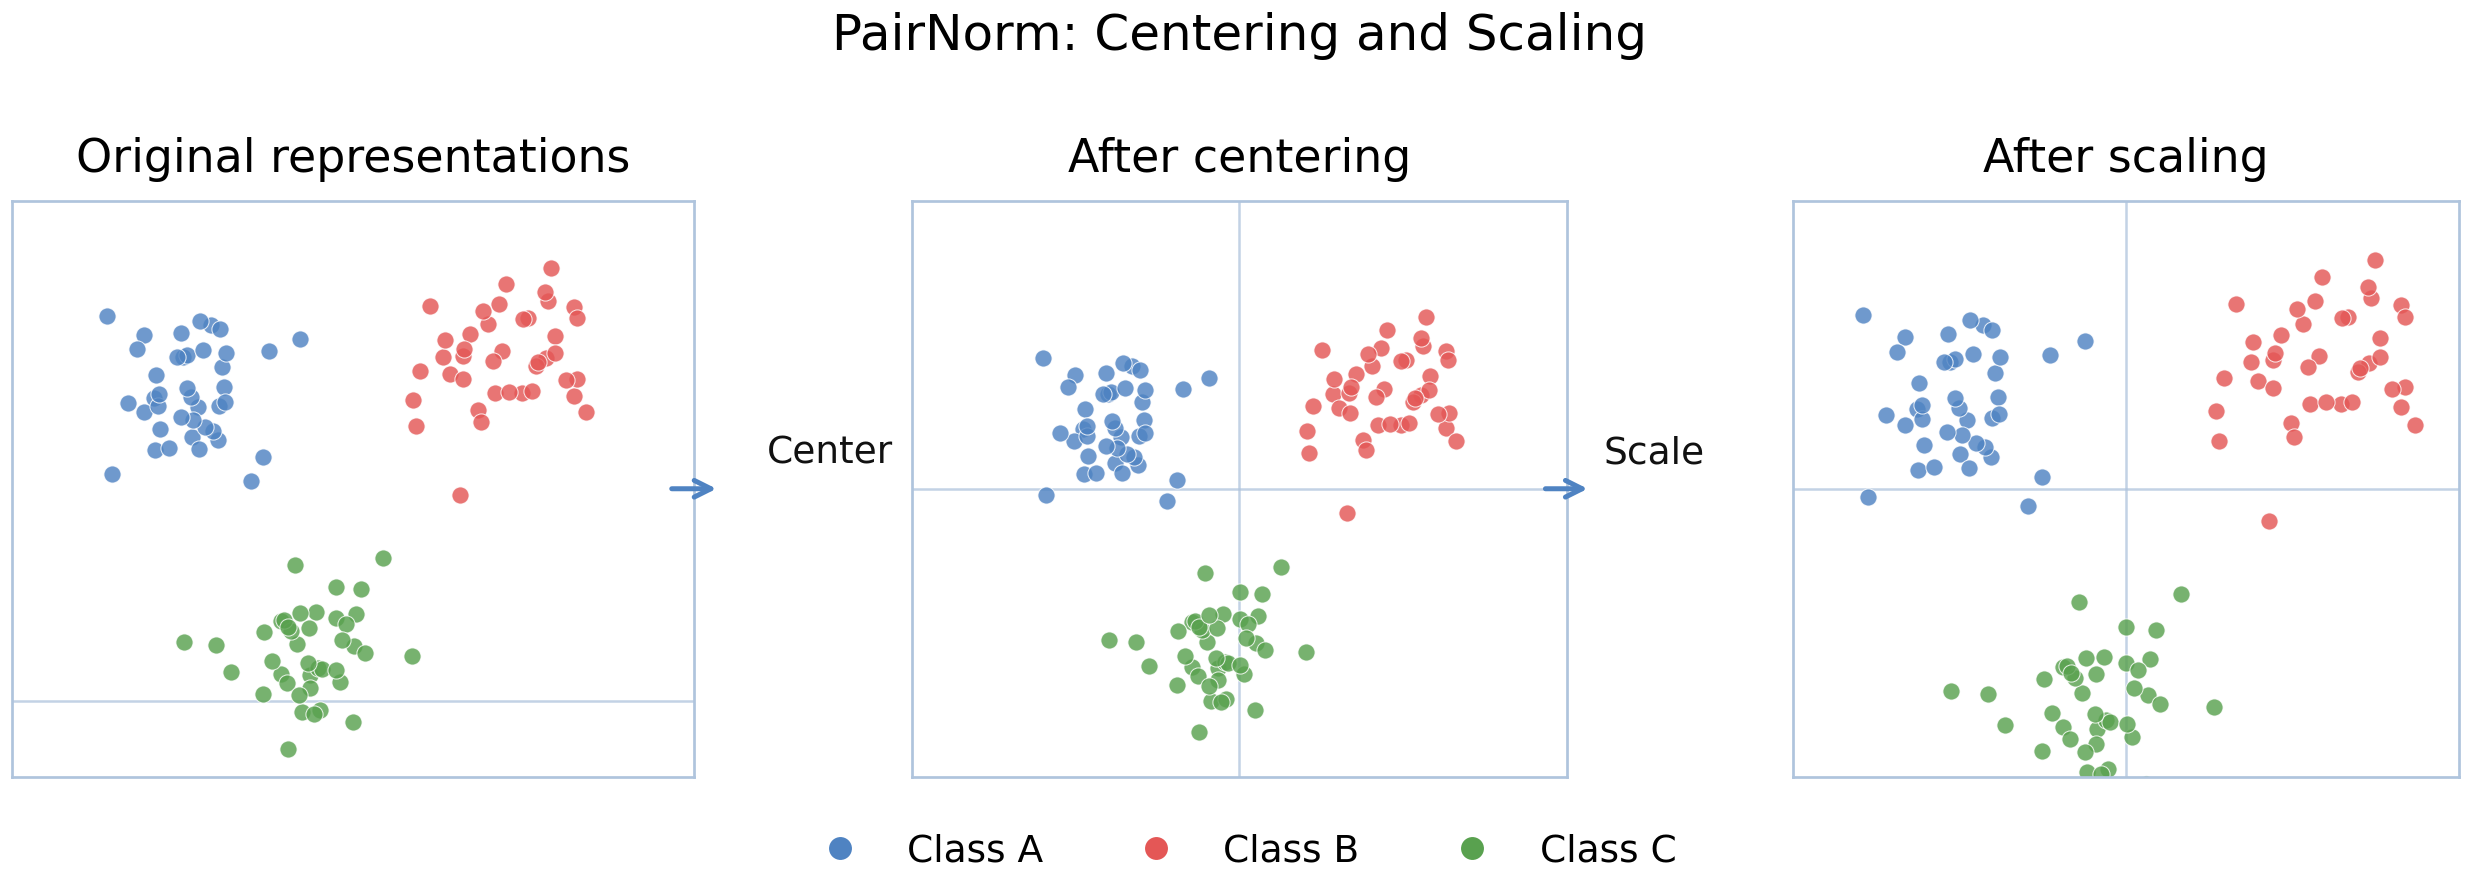
\includegraphics[
        width=0.95\textwidth,
        keepaspectratio
    ]{fig05_pairnorm.png}

   \caption{
    Conceptual effect of PairNorm on node-representation geometry.
    After message passing has reduced the global spread of the
    representations, PairNorm recenters them and rescales the
    representation matrix to a fixed global pairwise-distance scale.
    The operation constrains the overall geometry and does not
    preserve each individual pairwise distance.
}
    \label{fig:pairnorm-concept}
\end{figure}


% ============================================================
% 3 Experimental Methodology
% ============================================================

\section{Experimental Methodology}
\label{sec:methodology}


% ============================================================
% 3.1 Real-World Datasets
% ============================================================

\subsection{Real-World Datasets}
\label{sec:real-world-datasets}

% To be written later.


% ============================================================
% 3.2 Evaluation Protocol
% ============================================================

\subsection{Evaluation Protocol}
\label{sec:evaluation-protocol}

% To be written later.


% ============================================================
% 3.3 Oversmoothing Diagnostics
% ============================================================

\subsection{Oversmoothing Diagnostics}
\label{sec:oversmoothing-diagnostics}

% To be written later.


% ============================================================
% Bibliography
% ============================================================

\clearpage

\bibliography{references}


\end{document}